\chapter{Description and analysis of existing test framework} 
% Main chapter title

\label{Chapter3} % Change X to a consecutive number; for referencing this chapter elsewhere, use \ref{ChapterX}

%----------------------------------------------------------------------------------------
%	SECTION 1
%----------------------------------------------------------------------------------------

\section{Description of existing test framework}
Description and analysis of existing LBARD framework

\begin{itemize}
    \item Go into much more detail than lit review
    \item Since we are extending, need to fully explain and understand
    \item Analysis of log files
    \item how it functions
\end{itemize}

Two emulators for the Serval mesh exist. 
The first was built to test the functionality of the Serval mesh in its early days; when nodes were purely communicating over WiFi. 
This emulator is able to emulate multiple aspects of the serval-dna software, from validating the database integrity to \todo{add more} to simulating WiFi communication between Serval nodes. 
Later, once LBARD was added to the Serval project, a second emulator was built. 
This emulator performed similar functions to that of the serval-dna; testing internal LBARD functionality, and emulating radio communication between Serval nodes. 
While the LBARD emulator serves as an extension to the serval-dna emulator - extending and overwriting functionality - there is no ability to run tests that feature both WiFi and radio links.
\\
\emph{Unless otherwise specified, when talking about the test framework in this document, we will be talking about the LBARD test framework.}
\todo{add: what it is, how it functions}
\\


The two emulators are both written as bash shell scripts, where the LBARD test framework extends and overwrites several of the functions in the serval-dna emulator to get it to work with LBARD and fakeradio.
\todo{Add more about how it extends it, what the serval-dna test script does, etc.}
LBARD Emulator
\begin{itemize}
    \item Bash script
    \item 
\end{itemize}



\subsection{Aims of test framework}
What it /wants/ to be doing

Why it exists


\subsection{Functionality}
The LBARD test framework is able to run a vast range of defined tests, and because of this, is able to test large portions of the functionality of the LBARD software.

The test suite runs multiple instances of the actual serval-dna software, with LBARD processes running on top of this, and each instance is networked together through the 'fakeradio' software.
The fakeradio software monitors the LBARD radio outputs of each of the LBARD interfaces, and sends the packets it receives to the inputs of each of the LBARD radio input files, dependent on the rules defined when starting the fakeradio program.
The rules that can be sent to fakeradio allow test creators to define network layouts by denying all traffic between nodes unless specified otherwise, allowing for any topology to be defined.


When a test is run, the test suite starts the specified number of serval instances, each with their own separate databases, configurations, and log files.
Then, LBARD instances are started for each of these instances, running simulated radio hardware (RFD900, BarrettHF, etc.) as defined in the test definition.
Finally, fakeradio is started and begins to listen to the output files of each of the LBARD interfaces.
Once a test is concluded, the framework collects all of the log files and stdin/stdout/stderr of the serval intstances, LBARD instances, and fakeradio.
These are then collated into a single test log file, with every piece of data timestamped.
This way of running the tests has several benefits for the purpose of this Honours project; firstly, the test framework is running the real software that runs in a real-world scenario, with only the radio and wifi communications being simulated; secondly, the framework collates all of this data into a single log file, greatly minimising the work that needs to be done in later stages of this project to extract events in a test from multiple log files.

\subsection{Defining Tests}
Tests are defined in either the lbard or lbard\_size\_tests file. 
These are both bash files that source the lbard test framework, and simply define what tests are to be run.
Tests are comprised of three basic components; a doc string with a brief description of what the test does, a 'setup' function that sets up the test environment, and finally, a 'test' function, that is run when the test is run.
The doc string is used when running tests and serves as feedback to the tester as to what test is currently being run.
The setup function is run before the test is conducted. This function serves to set up any necessary configurations for the running of this test. This is where the fakeradio rules are defined, files added to Serval instances, and any other necessary setup for a test.
Finally in the test function, the conditions for a successful test are defined. Once this function completes (or an error/fail/timeout is encountered), the test concludes.


This can be seen in Figure \ref{fig:testDefinition}. 
In this example, setup function defines the fakeradio rules, then adds a single file of 50 bytes to the instance A. 
In the test function, a function 'all\_bundles\_received' is defined, that simply checks if instance B received a bundle with the specified bundle ID and version. 
The test then waits until this bundle is received. 
If this bundle is received before the default timeout, the test will pass.

\begin{figure}
    \begin{centering}
        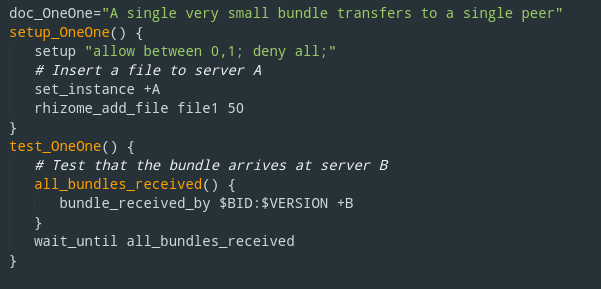
\includegraphics[width=14cm,height=20cm,keepaspectratio]{Figures/testdefinitionexample.png}
        \caption{Example of LBARD test definition}
        \label{fig:testDefinition}
    \end{centering}
\end{figure}


\begin{itemize}
    \item \# Intro, brief explanation
    \item \# The features it has
    \begin{itemize}
        \item \# Logging all info
        \item \# run the actual software
    \end{itemize}
    \item \# Defining tests
    \item What it currently does (what tests can do)
    \item What tests already exist (show all? list notable?)
    \item How the tests work
    \begin{itemize}
        \item Setting up virtual devices
        \item Running serval-dna test suite underneath
        \item Simulates links and traffic between
        \item Logs data transfer along those links
    \end{itemize}
    \item Running the tests (feedback, PASS/FAIL/ERROR)
\end{itemize}


\subsection{Outputs}
When a test is run a log file is produced. 
This log file contains the outputs from multiple processes. 
The log file contains the outputs (stdout) and error messages (stderr) from: \begin{itemize}
    \item the test script,
    \item fakeradio and, 
    \item all the fakeradio and LBARD forks, 
    \todo{Can we also get logs from the WiFi transfer?}
\end{itemize}

As we can see, all components of the LBARD test framework are logged.
The end result of this is that a single log file with the information from all components of the framework.
\todo{Rewrite this garbage}



\begin{itemize}
    \item Log files
    \item Format of them
    \item What information is found within
\end{itemize}



\section{Limitations}
What it doesn't do
\begin{itemize}
    \item No ability to have dual link types; ie. a node cant send/receive WIFI as well as send/receive UHF. Means that all topologies are limited to a single type of radio type. \emph{Not realistic at all for a real-world situation}
    \item Cannot currently use the serval-dna WiFi simulator ALONGSIDE LBARD-tests fakeradio
    \item Does not output topology information
\end{itemize}

\section{How to improve}
\begin{itemize}
    \item Talk about what I'll be doing to improve the framework
    \item What features it needs to suit this honours
\end{itemize}


\begin{itemize}
    \item Add new lbard/tests file specifically for topologies: no point in rendering .dot files for the small setup stuff
    \item Add to topology test file the ability to have multiple link types: we're doing combination radio types in the real world so we need to cover that
\end{itemize}
